\documentclass[12pt,letterpaper]{article}
\usepackage[utf8]{inputenc}
\usepackage{amsmath}
\usepackage{amsfonts}
\usepackage{amssymb}
\usepackage{graphicx}
\graphicspath{ {figures/} }
\usepackage{array}
\usepackage{caption}
\usepackage{float}
\usepackage{todonotes}
\usepackage{appendix}
\usepackage[backend=biber, style=numeric, citestyle=numeric]{biblatex}
\usepackage{tabularx}
\usepackage[margin=1in]{geometry} 
\usepackage{textcomp} %textdegree
\usepackage[space]{grffile} %permits space in includegraphics
%\usepackage{lipsum}
%%%%%%%%%%%%%%%%%%%%%%%%%%%%%%%%%%%%%%%%%%%%%%%%%%%%%%%%%%%% Preamble
\addbibresource{ref.bib}
\bibliography{B:/eskalvarado/Google Drive/University/2nd year - 2nd semester/Differential Equation/Couple First Order Differential Equations/ref.bib}

\renewcommand{\listfigurename}{Figures}
\renewcommand{\listtablename}{Tables}
%\setcounter{secnumdepth}{0}
\setcounter{tocdepth}{2}
\setlength{\parindent}{0pt}
\setlength{\parskip}{1em}
\rmfamily

\author{Edvin Alvarado Velez}
\title{Solution for Coupled First Order Differential Equations}

\newcommand{\vectors}[2]{
	\begin{pmatrix}
		#1 \\ #2
	\end{pmatrix}
}

\newcommand{\smatrix}[4]{
	\begin{pmatrix}
		#1 & #2 \\ #3 & #4
	\end{pmatrix}
}

\newcommand{\dmatrix}[4]{
	\begin{vmatrix}
		#1 & #2 \\ #3 & #4
	\end{vmatrix}
}

\newcommand{\bmath}[1]{\text{\textbf{#1}}}
%%%%%%%%%%%%%%%%%%%%%%%%%%%%%%%%%%%%%%%%%%%%%%%%%%%%%%%%%%%% Document
\begin{document}

	\maketitle
	
	\pagenumbering{gobble}
	% \tableofcontents	
	% \begingroup
	% \let\clearpage\relax %lets you join both lists somehow
	% \listoffigures	
	% \listoftables
	% \endgroup
	\clearpage
		
	\pagenumbering{arabic}

	\section{Vector Method}

		Having the following system of differential equations

		\begin{align*}
			\frac{\mathrm{d}x_1}{\mathrm{d}t} = a x_1 + b x_2 \\
			\frac{\mathrm{d}x_2}{\mathrm{d}t} = c x_1 + d x_2 
		\end{align*}

		It can be written as:

		\begin{equation}
			\frac{\mathrm{d}}{\mathrm{d}t} \vectors{x_1}{x_2} = \smatrix{a}{b}{c}{d} \vectors{x_1}{x_2}
		\end{equation}
		\label{og}

		The 2x2 matrix would be the characteristic matrix known as \textbf{M}. The roots of the equation can be found with:

		\begin{equation}
			\begin{vmatrix}	\text{\textbf{M}}-r \text{\textbf{I}} \end{vmatrix} = \left| \smatrix{a}{b}{c}{d} - r \smatrix{1}{0}{0}{1} \right| = \dmatrix{a-r}{b}{c}{d-r} = 0
		\end{equation}
		\label{characteristic matrix}

		\begin{align*}
			(a-r)(d-r) - bc = 0 \\
			r^2 -(a+d)r + ad -bc = 0 
		\end{align*}

		\begin{equation}
			r_{1,2} = \frac{(a+d) \pm \sqrt{(a+d)^2-4(ad-bc)}}{2}
		\end{equation}
		\label{roots}

		\subsection{General Solutions}

			As long as the square root is greater or equal to zero then the general solution is:

			\begin{equation}
				\bmath{x} =  \bmath{u}_1 e^{r_1 t} + \bmath{u}_2 e^{r_2 t}
			\end{equation}

			However if the root is complex $\alpha + \beta i$:

			\begin{equation}
				\bmath{x} =  \bmath{u}_1 e^{\alpha_1 t} (\cos{\beta_1 t} + i \sin{\beta_1 t}) +\bmath{u}_2 e^{\alpha_2 t} (\cos{\beta_2 t} + i \sin{\beta_2 t})
			\end{equation}

			The root will only be complex if the square root is negative. Therefore, let's verify when this happens:

			\begin{align*}
				(a+d)^2-4(ad-bc) < 0 \\
				% (a-d)^2 +4bc < 0 \\ 
				% bc > \frac{(a-d)^2}{4}
			\end{align*}

			A 3D Model can be done by joining the symmetric independent variables such as \emph{b} with \emph{c} and \emph{a} with \emph{d}. They're symmetric or conjoined in such a way that two random values can be assgined to each element to a pair and it would give the same result as if you had assigned the values in reverse. In mathematical notation:

			\begin{equation}
				f(a,b,c,d) = (a+d)^2-4(ad-bc)
			\end{equation}

			\begin{equation}
				f(a,x_0,x_1,d) = f(a,x_1,x_0,d)
			\end{equation}

			This is also true for the pair \emph{a} and \emph{d}. This is thanks the variables being multiplied and/or being inside a even exponential. So the model is the following:

			\begin{align*}
				A &= ad \\ 
				B &= bc \\
				\\
				f(a,b,c,d) &= (a+d)^2-4(ad-bc) \\
				&= \left( \frac{ad}{d} + d \right)^2 - 4(ad-bc) \\
				f(A,B,d) &= \left( \frac{A}{d} + d \right)^2 - 4(A-B)
			\end{align*}

			Although \emph{d} couldn't be fully eliminated, as \emph{A} includes variable \emph{d}, The 3D model should still accurately portray the function of the square root.

			% If \emph{b} or \emph{c} is negative and it fulfills the former equation then the roots will be complex.

			\begin{figure}[H]
				\centering
				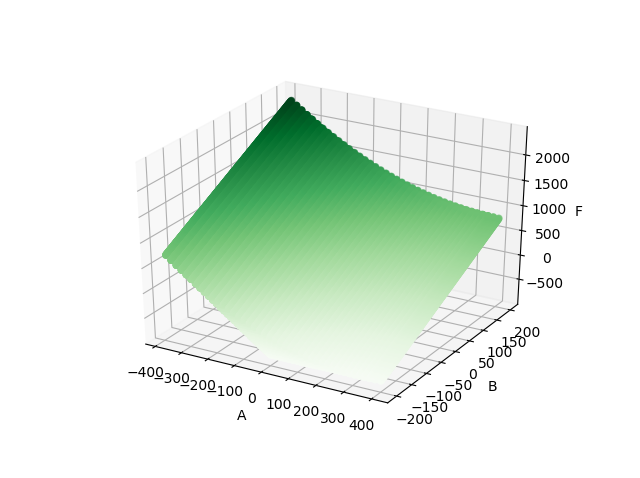
\includegraphics[width=0.8\textwidth]{3Dmodel.png}
				\caption{Python Model}
				\label{fig:3dmodel}
			\end{figure}

		
		\subsection{Roots of Equation}

			Once then roots (eigevalues) are known, we need to find the eigenvectors $U_i$. Substituting the roots to equation \ref{characteristic matrix}:

			\begin{align*}
				\smatrix{a-r_1}{b}{c}{d-r_1} \vectors{u_1}{u_2} = 0 \\ 
				\smatrix{a-r_2}{b}{c}{d-r_2} \vectors{u_1}{u_2} = 0 
			\end{align*}

			You can verify if the matrix is correct if it looks like this:

			\begin{equation*}
				\smatrix{p}{q}{p}{q}
			\end{equation*}

			in such a way that:

			\begin{equation*}
				(a-r_1) u_1 + b u_2 = c u_1 + (d-r_1) u_2
			\end{equation*}

			Now to solve for the eigenvectors using arbitrary number $(s_i)$:

			\begin{align*}
				(a-r_1) u_1 + b u_2 = 0 \\
				u_2 = s_1 \\
				u_1  = -s_1 \frac{b}{a-r_1} \\
				\vec{u}_1 = s_1 \vectors{-\frac{b}{a-r_1}}{1}
			\end{align*}

			\begin{align*}
				(a-r_2) u_1 + b u_2 = 0 \\
				u_1 = s_2 \\
				u_2  = -s_2 \frac{a-r_2}{b} \\
				\vec{u}_2 = s_2 \vectors{1}{-\frac{a-r_2}{b}}
			\end{align*}

			The General Solution wil be:

			\begin{equation}
				\vectors{x_1}{x_2} = s_1 \vectors{-\frac{b}{a-r_1}}{1} e^{r_1 t} + s_2 \vectors{1}{-\frac{a-r_2}{b}} e^{r_2 t}
			\end{equation}

	\section{Substitution method}

		Using the same system of differential equations We use the first equation to substitute $x_2$ of the second equation:

		\begin{equation}
			x_2 = \frac{1}{b} \left( \frac{\mathrm{d}x_1}{\mathrm{d}t} - ax_1 \right)	
		\end{equation}
		\label{eq:x2}

		\begin{align*}
			\frac{1}{b} \frac{\mathrm{d}}{\mathrm{d}t} \left( \frac{\mathrm{d}x_1}{\mathrm{d}t} - ax_1 \right) = cx_1 + \frac{d}{b} \left( \frac{\mathrm{d}x_1}{\mathrm{d}t} - ax_1 \right) \\
			\frac{\mathrm{d}^2 x_1}{\mathrm{d}t^2} - (a+d) \frac{\mathrm{d}x_1}{\mathrm{d}t} + (ad-bc)x_1 = 0 \\
			r^2 -(a+d) r + (ad-bc) =0
		\end{align*}

		Notice the quadratic formula of this equation is identical to equation \ref{roots}. \todo{wrong reference} 

		\begin{align*}
			x_1 = s_1 e^{r_1 t} + s_2 e^{r_2 t} \\
			\frac{\mathrm{d}x_1}{\mathrm{d}t} = s_1 r_1 e^{r_1 t} + s_2 r_2 e^{r_2 t}
		\end{align*}

		Substituting in equation \ref{eq:x2}  \todo{wrong reference}  the general solution of $x_2$ can be derivated:

		\begin{align*}
			x_2 &= \frac{1}{b} \left[ s_1 r_1 e^{r_1 t} + s_2 r_2 e^{r_2 t} - s_1 e^{r_1 t} - s_2 e^{r_2 t}\right] \\
			&= s_1 \frac{r_1 - 1}{b} e^{r_1 t} + s_2 \frac{r_2 - 1}{b} e^{r_2 t}
		\end{align*}

		So the general solution is:

		\begin{equation}
			\vectors{x_1}{x_2} = s_1 \vectors{1}{\frac{r_1 - 1}{b}} e^{r_1 t} +s_2 \vectors{1}{\frac{r_2 - 1}{b}} e^{r_2 t}
		\end{equation}

	\section{Example}

		\begin{equation}
			\frac{\mathrm{d}}{\mathrm{d}t} \vectors{x_1}{x_2} = \smatrix{-0.5}{0.5}{0.5}{-0.5} \vectors{x_1}{x_2}
		\end{equation}

		\begin{equation}
			\vectors{x_1}{x_2} = s_1 \vectors{1}{1}  + s_2 \vectors{1}{-1} e^{ - t}
		\end{equation}

	\section{Conclusion}

		So this two should give the same result. However, I suggest the Vector Method instead of Substitution as it's simpler and less prone to mistakes. 

	%\cite{main}
	\nocite{*}
	\printbibliography

	%\clearpage
	
%	\appendix
%	\chapter{aaa}
%	\section{bbb}
	
\end{document}

